\documentclass[11pt]{scrreprt}

% default stuff 
\usepackage[utf8]{inputenc}
\usepackage{ngerman}
\usepackage{hyperref}
\linespread{1.25}
\usepackage{listings} 
\usepackage{graphicx}
\usepackage[usenames,dvipsnames,table]{xcolor}
\usepackage{tikz}
\usepackage{multirow} %für Multirow Tabellen

\definecolor{a}{HTML}{FDF9EF}
%Hintergrund Text
\definecolor{b}{HTML}{F4F1E5}
%Hintergrund Body
\definecolor{c}{HTML}{544738}
%Schriftfarbe
\definecolor{d}{HTML}{98BF21}
%Buttonflächen
\definecolor{e}{HTML}{C2C5BE}
%Footerbackground
\definecolor{f}{HTML}{BBBBBB}
%Schrift in Tagcloud
\definecolor{g}{HTML}{303030}
%Tagcloud

\lstset{numbers=left, numberstyle=\tiny, numbersep=5pt} \lstset{language=Perl}
\setcounter{tocdepth}{2}
%Kopf- und Fußzeile
\usepackage{fancyhdr}
\pagestyle{fancyplain}
\fancyhf{}

%Kopfzeile links bzw. innen
\fancyhead[L]{\nouppercase{\leftmark}}
%Kopfzeile rechts bzw. außen
\fancyhead[R]{\today}
%Linie oben
\renewcommand{\headrulewidth}{0.5pt}

%Fußzeile links bzw. innen
\fancyfoot[L]{moosr}
%Fußzeile rechts bzw. außen
\fancyfoot[R]{\thepage}
%Linie unten
\renewcommand{\footrulewidth}{0.5pt}

% beautiful colors like redrubin ;)

%titlepage will das so
\newcommand{\HRule}{\rule{\linewidth}{0.5mm}}

% let the fun begin
\begin{document}


%\title{Studienarbeit Webtechnologie und Webmarketing mit OpenSource Software \\
%    \includegraphics[scale=0.5]{./elchlogo.png} \\
%    \normalsize{A music metadata search engine.}
%}
%\author{Dozent: Dr. Alois Kastner-Maresch\\
%Christopher Pahl, Christoph Piechula}
%\date{\today}

\begin{titlepage}
\begin{center}

% Upper part of the page
\textsc{\LARGE  Hochschule Hof, University of Applied Sciences}\\[1.5cm]
\textsc{\Large Webtechnologie und Webmarketing mit OpenSource Software}\\[0.5cm]


% Title
\includegraphics[scale=0.4]{./gfx/elchlogo}\\[1cm]    
\HRule \\[0.4cm]
{ \huge \bfseries A music metadata search service}\\[0.4cm]

\HRule \\[1.5cm]

% Author and supervisor
\begin{minipage}{0.4\textwidth}
\begin{flushleft} \large
\emph{Beteiligte Studenten:}\\
Christopher \textsc{Pahl}\\
Christoph \textsc{Piechula}
\end{flushleft}
\end{minipage}
\begin{minipage}{0.4\textwidth}
\begin{flushright} \large
\emph{Dozent:} \\
Dr. Alois \textsc{Kastner-Maresch}
\end{flushright}
\end{minipage}

\vfill

% Bottom of the page
{\large \today}

\end{center}

\end{titlepage}

\tableofcontents

\chapter{Die Idee}

Im Netz gibt es eine riesige Menge an Seiten die sich darauf spezialisiert
haben Informationen jeglicher Art zu Musikstücken, Künstlern und ähnlichem zu
liefern.
\\
Die Reichweite geht dabei von Songtexten bis hin zu Tagging-Informationen die von
Musikabspielprogrammem ausgelesen werden kann. Es gibt Streamingdienste wie last.fm,
oder Spotify die neben der eigentlichen Musik auch entsprechende Metadaten anbieten. 
Im Falle von last.fm sogar mit einer gut nutzbaren Webschnittstelle.
\\
Allerdings sind die ganzen Informationen mehr oder minder über das ganze Web
fragmentiert. Last.fm bietet lediglich Coverart und Künstlerbilder an, 
lyrics.wikia.com nur Lyrics und ein anderer Provider nur Biographien und
Reviews.
\\
Unsere Idee ist nun eine Metadatensuche zu bauen, die möglichst viele
Metadatentypen bündelt und dabei auch über eine Web-API nutzbar ist.
\\
Um diese Idee abzurunden wollen wir uns einen Namen in der Indie Musik Szene
schaffen und bieten neben der Suchdienstleistung zugleich einen ,,Treffpunkt'' für Indie
Musik Liebhaber, Liedermacher und freischaffende Künstler an.

\chapter{Untersuchung (20 Fragen)}

\label{wettbewerb}
\section{Welche besonderen Eigenschaften, Stärken, Alleinstellungsmerkmale hat (m)eine Leistung?}
Unsere Dienstleistung bietet eine zentrale Anlaufstelle für Indie Musik
Liebhaber, Liedermacher und Künstler und kombiniert diese mit einer Metadaten Suchmaschine
die Cover-Art Suche, Songtext-Suche, Biographie-Suche und Artistphoto-Suche in
einer Dienstleistung bündelt.
\\
\\
Anbieter mit ähnlichen Dienstleitungen: \\

\begin{itemize}
    \item \url{http://www.allcdcovers.com}
    \item \url{http://www.albumart.org} (keine soziale Komponente)
    \item \url{http://lyrics.wikia.com/Lyrics\_Wiki}
    \item \url{http://www.last.fm}
\end{itemize}

\section{Welche besonderen Alleinstellungsmerkmale und Vermarktungskonzepte haben Mitbewerber?}
\paragraph{Last.fm}
Der Anbieter Last.fm spezialisiert sich hauptsächlich auf Musikstreaming.
Desweiteren bietet er eine Metadatenschnittstelle an, die Artist-Biographien,
Cover-Art und Artist-Photos liefern kann. Kompatible Clients und Webseiten können
daher diese anzeigen. Zudem bietet er eine soziale Komponente an, indem pro User
ein Profil vorhanden ist, auf dem einsehbar ist was dieser gerade hört bzw. mag.

\paragraph{allcdcovers}
Dieser Anbieter hat sich auf besonders hochauflösende Cover-Art Images
spezialisiert. Außerdem bietet er zudem Bilder von der CD Rückseite und dem
Inlet an. Er ist vollkommen Community-basiert.

\paragraph{albumart}
Der Anbieter Albumart ähnelt unserem Suchangebot noch am ehesten. Allerdings
beschränkt er sich lediglich auf CD und DVD Cover-Art. Er bietet zudem eine API.

\paragraph{lyrics.wikia}
Dieses Angebot ist in einer Wiki-ähnlichen Struktur organisiert. Leider bietet
dieser Anbieter nur Songtexte an. Allerdings verlinkt er auf andere Angebote und
integriert soziale Dienste wie Twitter und Facebook.
\\
\\
Wir sollten erwähnen dass es noch eine große Anzahl weiterer Webseiten gibt.
Allerdings haben wir die oberen exemplarisch als Vergleich ausgewählt.

\section{Wie können wir unsere Leistung durch eine Spezialisierung abgrenzen und unsere Stärken optimal zur Geltung bringen?}
Unsere Dienstleistung konzentriert sich auf die Bereitstellung einer
leichtgewichtigen Webschnittstelle die sowohl andere Webseiten als auch
Desktopclients nutzen können. Das Hauptaugenmerk liegt hier auf einer besonders
guten Dokumentation sowie einer einfachen Integration der Dienste in
verschiedenen externen Produkten.
\\
\\
Allerdings versteht sich unser Angebot als eine Art ,,Metaprovider``, der sich
auf andere Dienstleister wie beispielsweise last.fm stützt und diese bündelt.
\\
Als Anlaufstelle für eine große Community fühlen wir uns verpflichtet diese
neben unserem Suchdienst über Neuigkeiten jeglicher Art auf dem Laufenden zu
halten.
\\
\\
Auf technischer Seite legen wir großen Wert auf Transparenz und die Integration
freier Software. So steht der Quellcode der Anwendung offen auf Github\footnote{\url{https://www.github.com/studenkittens/flascat}} zur
Verfügung. 



\section{Was ist die erfolgversprechendste Zielgruppe?}
Als Zielgruppe sehen wir primär Musikinteressierte Benutzer und Anbieter von
Musik-Abspielsoftware (und damit deren Nutzerbasis).
Die Zielgruppe ist prinzipiell ein junges experimentierfreudiges Publikum das
sich schnell für Neues begeistern lässt.

\section{Welche Medien nutzt die Zielgruppe?}
Primär nutzt die Zielgruppe das Internet. Andere Medien sind für unsere
Dienstleistung zu vernachlässigen.

\section{Wer sind die wichtigsten Meinungsführer?}
Frage trifft auf unsere Dienstleistung nicht zu, da es in dem Sinne keine
Meinungsführer gibt.

\section{Was sind die brennenden Probleme der Zielgruppe?}
Die Zielgruppe hat das Problem Metadaten an einer zentralen Stelle im Netz
aufzufinden. Unsere Dienstleistung soll diese Angebotslücke schließen und
zusätzlich als Treffpunkt für gleichgesinnte Musikliebhaber und freischaffende
Künstler dienen.
\\
\\
Wie oben bereits ist die Verteilung der Communities stark dezentral. Wir wollen
das nach Möglichkeit soweit wie möglich zentralisieren und bieten ein Forum 
sowie links auf andere Seiten.


\section{Welche Trojanische Pferde können wir entwickeln?}
Im Moment gibt es kein Angebot das verschiedene Metadaten maschinenlesbar 
in einem Angebot bündelt. Unser Angebot kann auf anderen Webseiten leicht durch
die leichtgewichtige Webschnitstelle eingebunden werden.
\\
\\
Ein zwingender Nutzen würde sich für Musicplayer ergeben, da dort 
Client-Bibliotheken für unseren Service zur Verfügung stehen.

\section{Welche Überraschung können wir Meinungsführern bieten?}
Frage trifft auf unsere Dienstleistung nicht zu, da keine Meinungsführer
vorhanden.

\section{Wie können wir ein Angebot mit PR bekannt machen und nicht nur durch Anzeigenwerbung?}
Durch den Einsatz von sozialen Medien wie Twitter oder Facebook kann ein
positives Meinungsbild suggeriert werden. Desweiteren kann der Service von
verschiedenen Fachseiten getestet und empfohlen werden. Aufgrund der hohen 
Verfügbarkeit unserer Dienstleistung die sich über verschiedene soziale Netze
von Facebook bis hin zu Flickr streut sollte es problemlos möglich sein unsere
Dienstleistung einem breitem Publikum zugänglich zu machen.

\section{Welche Risiken gibt es dafür, dass die Zielgruppe die Leistung nicht nutzen könnte? Was kann potentielle Kunden eventuell abschrecken?}
Ein mögliches Risiko wäre eine zu komplexe Entwickler unfreundliche API. Um
dieses Risiko zu minimieren wird darauf geachtet die API und Seite nach offenen
Standards zum implementieren.
\\
\\
Für normale User hätte ein kompliziertes und überladenes Design eine
abschreckende Wirkung, weswegen wir uns hier auf Minimalismus konzentrieren.

\section{Welche Kooperationsstrategie können wir verfolgen?}
Da wir außer einem externen Shop und sozialen Diensten nicht auf andere Partner
zurückgreifen trifft die Frage nicht auf unser Angebot zu.

\section{Können wir einen Markennamen generieren?}
Diese Frage trifft nicht direkt zu da es sich bei moosr in erster Linie um ein
nicht kommerzielles Produkt handelt wo die Etablierung eines Markennamens
zweitrangig ist. 

\section{Ist eine Intel-Inside Strategie möglich?}
Ja, eine Intel-Inside Strategie wäre denkbar wenn verschiedene Musikplayeranbieter
moosr als Metadatensuchmaschine nutzen. Diese Situation könnte man durch die
Implementierung von Wrapperlibraries für verschiedene Programmiersprachen
positiv beeinflussen.
\\
\\
Mögliche ,,Intel-Inside''-Claims für Playeranbieter:
\begin{itemize}
    \item \it{My Player supports Moosrdata search!}
    \item \it{Moosr bringt's} - Englisch alternativ: \it{Moosr delivers}
    \item \it{Moosr inside}
\end{itemize}

\section{Welches Key-Visual / Key-Theme können wir verwenden?}
Eine weiche, helle Farbgebung mit grün/braun Farbtönen die ein skandinavisches
,,Feeling'' vermittelt um die zunehmend in letzter Zeit aus den skandinavischen
Ländern kommende Indie Musik Bewegung visuell zu  unterstreichen.
\\
\\
Weitere Details zum KeyVisual/Claim finden sich im entsprechenden Kapitel
\ref{keyvisual_claim}.

\section{Können wir eine Strategie entwickeln, wie wir mit PR und Vorträgen an die Zielgruppe oder deren Meinungsführer direkt rankommen?}
Die Frage trifft nicht auf unsere Dienstleistungen zu.

\section{Wie können wir einen Markenaufbau zum Nulltarif erreichen?}
Wir setzen auf Mundpropaganda, siehe nächste Frage.

\section{Wie können wir Mundpropaganda unterstützen?}
Bei genügend Mundpropaganda und positiver Rezession verbreitet sich die
Dienstleistung automatisch über verschiedene Plattformen und Distributionen.
\\
\\
Dies sollte bei der hohen Verfügbarkeit in sozialen Netzen und der engen Bindung
zur Community kein Problem darstellen.

\section{Welchen Claim sollten wir verwenden? Die treffende Message bewirkt Wunder!}
Als Claim wurde ,,moosr bringt's.'' gewählt. Da dies ein kurzer, einprägsamer
Begriff ist der unsere Dienstleistung auf den Punkt bringt. Wir informieren über
Neuigkeiten und liefern Metadaten.

\section{Welches Leitbild und welche Ziele verfolgen wir für die Ansprache der Zielgruppe?}
Frage trifft nicht auf unsere Dienstleistung zu.


\chapter{Keyvisual und Claim}
Beim Key-Visual wurde als Logo ein Elch mit Saiten und Musiknoten im Geweih
gewählt.
\\
Die Wahl eines Tieres als Logo ist hier leicht an das Vorbild Napster
angelehnt welches eine Katze mit Kopfhörern zeigt.

\begin{center}
    \includegraphics[scale=0.4]{./gfx/napster.jpeg}
\end{center}

Es wurde bewusst ein Elch
ausgewählt, dieser soll symbolisch die anfangs überwiegend aus den
skandinavischen Ländern antreibende Kraft der Indie Musik Bewegung visuell
darstellen. Desweiteren sollen die Saiten im Geweih den Zusammenhalt der
Communiy wiederspiegeln, der grimmige Blick ist eine ,,Kampferklärung'' an die
Mainstream Musik Branche. Der comichafte Ansatz soll hier primär ein junges
Publikum ansprechen.
\section{Key-visual}

\begin{center}
    \includegraphics[scale=0.4]{./gfx/elchlogo.png}
\end{center}
\section{Claim}
Claim siehe\ref{claim}.

\chapter{Markt und Wettbewerb}
Dieser Punkt ist bei uns Bestandteil der ,,20 Fragen''.
\\
\\
Siehe dazu Kapitel \ref{wettbewerb}.

\chapter{Finanzierung}

\section{Lizenz}
Primär ist es uns wichtig den Bekanntheitsgrad zu steigern und eine große
Community zu gewinnen welche auch daran interessiert ist die Dienstleistung
weiter auszubauen und zu verbessern. Die direkte Kommunikation zu der Community
soll eine Weiterentwicklung der Dienstleistung gewährleisten und dabei
gleichzeitig die Interessen der ,,Kunden'' wahren.
\\
Aus diesem Grund haben wir uns für Freie Lizezen entschieden um so jedem die
Möglichkeit zu bieten die Dienstleistung zu verbessern.
\\
Alle Quelltexte stehen unter GPLv3 Lizenz.
\begin{center}
\url{http://www.gnu.org/licenses/gpl-3.0.html}
\end{center}
Das \emph{Design} sowie alle weiteren
Medien unter der Creative Commons Lizenz.
\begin{center}
\url{http://de.creativecommons.org/ }
\end{center}

\section{Mögliche Finanzierungsszenarien}
Da unsere Dienstleistung nicht kommerziellen Ursprungs ist trifft diese Frage
nicht direkt zu.
\\
Als primäre Finanzierungsquelle um die Serverkosten zu decken bieten wir über
Drittanbieter wie 
\begin{center}
 \url{http://www.zazzle.de/} 
 \\
 \url{http://www.cafepress.de/}
\end{center}
Fanartikel wie T-Shirts, Aufkleber etc. an. Durch diese Maßnahme wird zusätzlich
als positiver Nebeneffekt Werbung geschaffen.
\\
Mögliche Einnahmequellen wären Spenden und mögliche kostenpflichtige API
Anpassungen für ,,Kunden'' kommerzieller Musikplayer und Contentanbieter. Wir
erhoffen uns durch die freigewählten Lizenzen, dass kommerzielle Dienstleister
ermutigt werden unseren Dienst zu finanzieren und somit zur Entwicklung direkt
oder indirekt beizutragen.
\\
Eine weitere Art der Finanzierung wäre indirekt denkbar, wenn wir Vereinbarungen
mit den unter der Kategorie \emph{Webshops} für Fanartikel und Tickets die Ver
\\
Der Dienst an sich ist prinzipiell selbsttragend, da außer den
Unterhaltungskosten für Domain und Server keinerlei laufende Kosten anfallen sollten.

\chapter{Konzept Web}

\section{Allgemein}

Unsere Dienstleistung konzentriert sich ähnlich der Unix Philosophie auf eine
bestimmte Tätigkeit und versucht diese möglichst gut zu realisieren. Aufgrund
dieser Tatsache ist es uns sehr wichtig den User nicht mit ,,Thematikfremden''
Themen zu nerven. Aufgrund unserer Spezialisierung werden fachfremde Kategorien
wie z.B. der Fanartikel Webshop an Drittanbieter ,,outgesourct''.
\\
\\
Um eine einfache sowie angenehme Usability zu gewährleisten konzentrieren wir
uns sehr stark darauf das \emph{Design} nach dem KISS-Prinzip so einfach wie
möglich zu halten und den Benutzer nicht mit Werbebannern oder sinnvollen
Informationen zu belästigen.

\newpage

\section{Farbklima}
Das an den Key-Visual angepasste Farbklima sieht wie folgt aus:

\begin{table}[h!]
\centering
\begin{tabular*}{\textwidth}{lll|l}

    Farbe & Name & Farbwerte & Einsatzgebiet \\
    \hline
    
\multirow{3}{*}
    {
    
\begin{tikzpicture}
        \draw [line width=0.5pt,fill=a]
        (0,0) -- (1.2,0) -- (1.2,1.2) -- (0,1.2) -- cycle;
    \end{tikzpicture}
    }
    & a & HEX \#FDF9EF & Hintergrundfarbe für Contentbereich\\
    & & RGB 253, 249, 239 \\
    & &  \\
    \hline

\multirow{3}{*}
    {
    
\begin{tikzpicture}
        \draw [line width=0.5pt, fill=b]
        (0,0) -- (1.2,0) -- (1.2,1.2) -- (0,1.2) -- cycle;
    \end{tikzpicture}
    }
    & b & HEX \#F4F1E5 &  Hintergrund \\ 
    & & RGB  244, 241, 229 & \\
    & &  \\
    \hline

\multirow{3}{*}
    {
    
\begin{tikzpicture}
        \draw [line width=0.5pt,fill=c]
        (0,0) -- (1.2,0) -- (1.2,1.2) -- (0,1.2) -- cycle;
    \end{tikzpicture}
    }
    & c & HEX \#544738 &  Standard Schriftfarbe \\
    & & RGB 84, 71, 56 & \\
    & &  \\
    \hline

\multirow{3}{*}
    {
    
\begin{tikzpicture}
        \draw [line width=0.5pt,fill=d]
        (0,0) -- (1.2,0) -- (1.2,1.2) -- (0,1.2) -- cycle;
    \end{tikzpicture}
    }
    & d & HEX \#98BF21 &   Buttonflächen \\
    & & RGB 152, 191, 33 & \\
    & &  \\
    \hline

\multirow{3}{*}
    {
    
\begin{tikzpicture}
        \draw [line width=0.5pt,fill=e]
        (0,0) -- (1.2,0) -- (1.2,1.2) -- (0,1.2) -- cycle;
    \end{tikzpicture}
    }
    & e & HEX \#C2C5BE &  Footer Hintergrundfarbe \\
    & & RGB 194, 197, 190 &\\ 
    & &  \\
    \hline
   
\multirow{3}{*}
    {
    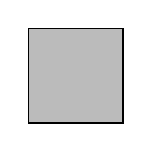
\begin{tikzpicture}
        \draw [line width=0.5pt,fill=f]
        (0,0) -- (1.2,0) -- (1.2,1.2) -- (0,1.2) -- cycle;
    \end{tikzpicture}
    }
    & f & HEX \#BBBBBB &  Tagcloud Schriftfarbe \\
    & & RGB 187, 187, 187  & \\
    & &  \\
    \hline
   
\multirow{3}{*}
    {
    
\begin{tikzpicture}
        \draw [line width=0.5pt,fill=g]
        (0,0) -- (1.2,0) -- (1.2,1.2) -- (0,1.2) -- cycle;
    \end{tikzpicture}
    }
    & g & HEX \#303030 &  Tagcloud Farbe \\
    & & RGB 48, 48, 48  & \\
    & &  \\

\end{tabular*}
   \caption{Farbschema}
   \label{t_colorscheme}
\end{table}

\section{Erläuterte Screenshots}

TODO

\chapter{Google Optimierung}

\section{Duplicate Content}
Mit mit Framework Flask lässt sich auf einfache Art und Weise \emph{duplicate
content} vermeiden. Hier zu kann technisch die \emph{url\_for()} Funktion
verwendet werden die einem die URL eines bestimmten Elements oder einer
View-Funktion zurückliefert. Im Folgenden Beispiel wird die Funktionsweise
erläutert:

\begin{verbatim}
                        @app.route('/hello')
                        def hello_func():
                            return 'Hello World'
\end{verbatim}

Die Url \url{http://www.moosr.org/hello} wir im Beispiel auf die Funktion
\emph{hello\_dunc()} gemappt. Beim Aufruf von \emph{url\_for('hello\_func')} wir
die Url \url{http://www.moosr.org/hello} zurückgeliefert. Durch den konsistenten
Zugriff über \emph{url\_for()} wird bei bei unserem Projekt
\emph{duplicate content} vermieden.



\section{Duplicate Content vermeiden}
Durch den Einsatz von Flask als Webframework haben wir volle Kontrolle über
die Festlegung einzelner URLs. 
\section{Content Seiten über Navigation erreichbar}


\section{Artikel über mehrere Seiten strecken}
\section{Festlegbare Linktexte}
\section{Einfache URLs erzeugen}


\section{Editierbare Metadaten}



\chapter{Technische Implementierung}
\section{Vorwort - technische Implementierung}
Als technische Grundlage für moosr wird ein Webframework verwendet, da dieses an
die benötigten Bedürfnisse (Suchmaschine) am relativ gut angepasst werden kann.

Als Webframework haben wir uns mit Absprache mit Herrn Prof. Dr. Alois
Kastner-Maresch auf das Python Microwebframework Flask geenigt da wir das
Framework in der Vorlesung \emph{Wiederverwendungsbasierte Entwicklung von
Systemen} in einer Studienarbeit erarbeiten und das dort gewonnene Wissen (Flask
und Python) praktisch in der Vorlesung ,,Webtechnologie und Webmarketing 
mit Open Source'' umsetzen möchten.

\subsection{Flask}
Das Microwebframework benutzt \emph{Jinja} als Template Renderengine und
\emph{Werkzeugs} als WSGI Middleware. Die Pakete selbst können mit pip gezogen
werden


Da die Webpräsentation primär als Dienstleistung zu sehen ist kommen bei der
Implementierung neben dem Framework selbst hauptsächlich auf die beiden
libraries \emph{libglyr} und \emph{sqlite3} zum Einsatz.

\subsection{libglyr}
Libglyr ist eine library zum auffinden von Musikmetadaten. 
\\
\url{https://github.com/sahib/glyr}


\subsection{sqlite3}
Sqlite3 ist eine sehr weit genutzte und bekannte embedded Datenbank, welche für
unseren Einsatz optimal ist.
\\
\url{http://www.sqlite.org/}

\chapter{Weiteres}

Unsere Dienstleistung soll sich hauptsächlich durch ihre Spezialisierung auf
Metadatensuche von der Konkurrenz abheben. 


\end{document}
